\documentclass[oneside, final, 14pt]{extreport}
\usepackage[utf8]{inputenc}
\usepackage[russian]{babel}
\usepackage{vmargin}
\setpapersize{A4}
\setmarginsrb{2cm}{1cm}{1cm}{1cm}{0pt}{0mm}{0pt}{13mm}
\usepackage{indentfirst}
\usepackage{amsmath}
\usepackage{graphicx}
\usepackage{wrapfig}
\sloppy

\begin{document}

\setcounter{chapter}{7}
\chapter{Пространственная обработка сигналов}
\tableofcontents

\section{Дилей. Эхо}
\subsection{Дилей}
\textbf{Дилэй} (англ. \emph{delay}~--- задержка)~--- эффект задержки звука; задержка происходит с помощью записи входного сигнала с последующим проигрыванием его через определённый период времени. Задержанный сигнал может воспроизводится либо один раз, либо несколько раз для создания повторяющегося звука похожего на распадающейся эхо.

До изобретения технологий задержки звука, для создания эффекта эха необходимо было производить запись в естественно звучащем помещении где присутствовало эхо, это доставляло большие неудобства для музыкантов и звукорежиссёров.

Первые эффекты дилэя создавались с помощью использования зацикленной магнитной ленты проигрываемой на магнитофоне (рис. \ref{pic-delay-01}). В начале ленты устанавливалась записывающая головка, а через определённый промежуток воспроизводящая, или несколько воспроизводящих для создания нескольких задержек. Путем сокращения или удлинения ленты и корректировкой записывающей и воспроизводящей головок, изменялся характер задержки.

\begin{figure}[h!]
  \centering
  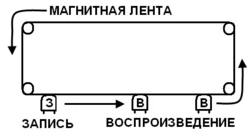
\includegraphics[width=0.75\textwidth]{pic-delay-01}
  \caption{Схема дилея на магнитной ленте}
  \label{pic-delay-01}
\end{figure}

\begin{figure}[h!]
  \centering
  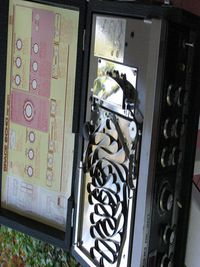
\includegraphics[width=0.4\textwidth]{pic-delay-02}
  \caption{Ленточный дилей Roland RE-201}
  \label{pic-delay-02}
\end{figure}

Тонкая магнитная лента не совсем подходила для непрерывной работы, поэтому время от времени лента должна была заменяться для сохранения верности и качества задержанного звука (рис. \ref{pic-delay-02}).

Другие популярные блоки как носитель использовали вращающийся магнитный барабан (к примеру дилэй \emph{Binson Echorec}, рис. \ref{pic-delay-03}). Это давало преимущество над магнитной лентой, потому как прочные барабаны были в состоянии работать в течение многих лет с небольшим ухудшением качества звука.

\begin{figure}[h!]
  \centering
  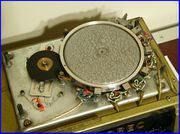
\includegraphics[width=0.5\textwidth]{pic-delay-03}
  \caption{Дилэй Binson Echorec на основе магнитного барабана}
  \label{pic-delay-03}
\end{figure}

Хотя аналоговые дилэи менее гибки чем цифровые и в целом имеют меньшее время задержки, несколько классических моделей, такие как \emph{Boss DM-2} по-прежнему ценятся за их "<теплое">, более естественное эхо. Кроме того, несколько компаний делают новые аналоговые дилэи, в их числе \emph{MXR Carbon Copy} и \emph{Ibanez AD9}, переиздавая свои педальные эффекты 1980-х годов.

Наличие недорогой цифровой обработки сигнала в конце 1970-х и 1980-х годов привело к разработке первых цифровых дилэев (рис. \ref{pic-delay-04}). Цифровые системы создавали задержку с помощью сэмплирования входного сигнала через аналого-цифровой преобразователь, после чего сигнал проходил через серию цифровых сигнальных процессоров, записывая сигнал в буфер хранения, а затем воспроизводя на основе установленных пользователем параметров. Задержки могут быть смешаны с сухим сигналом после или перед тем как он отправляется в цифро-аналоговый преобразователь.

Многие современные цифровые дилэи имеют обширный набор вариантов настроек, включая:
\begin{itemize}
  \item контроль времени до воспроизведения задержек сигнала (\emph{delay time});
  \item общий уровень обработанного сигнала по отношению к не обработанному (\emph{dry/wet});
  \item уровень на котором задержанный сигнал подается обратно в буфер, который будет снова повторяться ~--- так называемая \textbf{обратная связь} (\emph{feedback}).
\end{itemize}

\begin{figure}[h!]
  \centering
  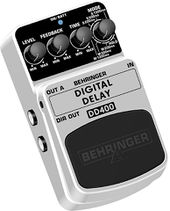
\includegraphics[width=0.4\textwidth]{pic-delay-04}
  \caption{Цифровой педальный дилэй Behringer Digital Delay DD400}
  \label{pic-delay-04}
\end{figure}

Следующим шагом развития цифровых аппаратных дилэев было появление программных систем задержек. Программные дилэи во многих случаях предлагают гораздо большую гибкость, чем даже самые лучшие цифровое оборудование. Большое количество системной памяти современных персональных компьютеров предлагает практически безграничный буфер для хранения звука, и более натуральные алгоритмы задержки, предлагая возможность смещения или внесения случайности в задержки, или вставку других звуковых эффектов в процесс обратной связи. Многие разработчики плагинов добавляют возможность подражания звукам ранних аналоговых устройств.

Наиболее часто эффект дилэя используется для создания эффекта эха. В популярной и электронной музыке, дилэй используется для создания плотных текстур. Очень большое время задержки 10 секунд или более используются для создания петель целых музыкальных фраз.

Также очень часто используется эхокомплекс, который создаёт повторяющиеся задержки синхронно с музыкальным ритмом, так что ноты комбинируются и рекомбинируются интересными способами.

\subsection{Эффекты \emph{Delay} в \emph{Adobe Audition}}
Команда \emph{Effects > Delay and Echo > Delay} открывает диалоговое окно эффекта \emph{Delay} (рис. \ref{pic-audelay-01}). В группах \emph{Left Channel} и \emph{Right Channel} находятся элементы настройки времени задержки для каждого стереоканала.

С помощью регулятора \emph{Delay Time} или непосредственно в поле ввода, расположенном справа от него, вы можете задать время задержки (единица измерения времени выбирается в поле \emph{Delay Time Units}). Состояние флажка \emph{Invert} определяет, будет ли сигнал инвертирован по фазе.

\begin{figure}[h!]
  \centering
  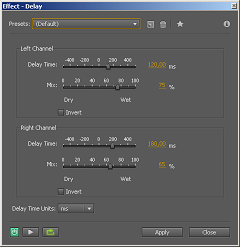
\includegraphics[width=0.5\textwidth]{pic-audelay-01}
  \caption{Окно эффекта Delay}
  \label{pic-audelay-01}
\end{figure}

Команда \emph{Effects > Delay and Echo > Analog Delay} открывает диалоговое окно эффекта \emph{Analog Delay} (рис. \ref{pic-audelay-02}). Данный эффект моделирует звучание устаревших аппаратных устройств.

Параметр \emph{Mode} задает тип моделируемого устройства, что, в свою очередь, определяет параметры эквализации и искажающего эффекта. Режимы \emph{Tape} и \emph{Tape/Tube} соответствуют по характеристикам старым ленточным и ламповым устройствам создающим эффект дилей, режим \emph{Analog}~--- более поздним электронным устройствам. Параметр \emph{Trash}~--- увеличивает искажения, а также усиливает нижние частоты, \emph{Spread}~--- задает ширину стереопанорамы.

\begin{figure}[h!]
  \centering
  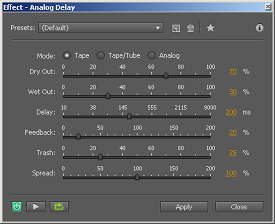
\includegraphics[width=0.5\textwidth]{pic-audelay-02}
  \caption{Окно эффекта Analog Delay}
  \label{pic-audelay-02}
\end{figure}

\subsection{Эффекты \emph{Delay} пакета \emph{Waves Platinum Native Bundle}}
В пакет \emph{Waves Platinum Native Bundle 4} входят два плагина, в которых реализованы многоотводные линии задержки:
\begin{itemize}
  \item \emph{SuperTap 2~--- Taps Mode} является двухотводной линией задержки;
  \item \emph{SuperTap 6~--- Taps Mode} является шестиотводной линией задержки.
\end{itemize}

Возможна установка времени задержки в миллисекундах или согласование задержки с темпом композиции, ручной ввод темпа или ритма повторений, модуляция времени задержки посредством низкочастотного генератора, панорамирование и эквализация сигнала каждого отвода по отдельности (рис. \ref{pic-wavesdelay-01}).

\begin{figure}[h!]
  \centering
  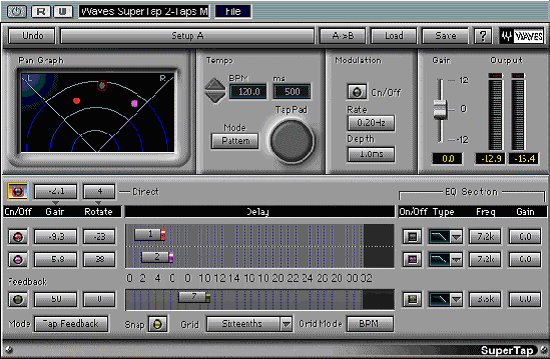
\includegraphics[width=0.75\textwidth]{pic-wavesdelay-01}
  \caption{Окно эффекта \emph{SuperTap 2~--- Taps Mode}}
  \label{pic-wavesdelay-01}
\end{figure}

Каждый отвод состоит из входной секции, регулятора времени задержки и эквалайзера.

Графический индикатор, расположенный вверху слева, позволяет наблюдать и изменять при помощи мыши одновременно уровень и положение на стереопанораме прямого сигнала и сигналов со всех отводов (каждый из них обозначен маркером своего цвета). Вместо того чтобы задавать значения параметров каждого из источников звука двумя регуляторам, можно перетаскивать мышью соответствующий маркер.

Расположенная рядом секция \emph{Tempo} обеспечивает ввод текущего темпа музыкального произведения в пределах от 40 bpm до 1200 bpm.

Специальная площадка \emph{TapPad} позволяет, реже или чаще щелкая на ней мышью, задавать темп (если кнопкой \emph{Mode} выбран режим \emph{Tempo}) или определенный ритмический рисунок (если выбран режим \emph{Pattern}).

В секции \emph{Modulation} расположен модулятор времени задержки, общий для всех отводов. Модуляция времени задержки дает возможность создавать эффекты, напоминающие хор.

\subsection{Эхо}
\textbf{Эхо} (англ. \emph{echo})~--- отражение звука, прибывающее к слушателю через некоторое время после прямого звука.

В природе эхо образуется в результате отражения звуковых волн от препятствий (домов, стен помещения, гор и т. п.). Различные спектральные составляющие звука по-разному отражаются от препятствий. Чем ниже частота, тем легче волна преодолевает препятствия. Высокочастотная волна не проходит сквозь препятствие, а отражается от него и частично поглощается. Кроме того, высокочастотные звуковые волны при распространении в воздухе затухают быстрее низкочастотных.

Основное отличие \textbf{эффекта эхо} от эффекта дилей состоит в том, что задержанные копии сигнала подвергаются дополнительной обработке~--- изменяется их спектр. Звук, обработанный эффектом эхо, имеет более натуральное звучание. Таким образом, эхо содержит смещенный во времени исходный сигнал, у которого будут ослаблены и низкие, и высокие частоты.

С помощью диалогового окна эффекта \emph{Effects > Delay and Echo > Echo} можно смоделировать описанные ранее условия (рис. \ref{pic-auecho-01}). Регулятор \emph{Delay Time} задает время, на которое будет задержан сигнал. Регулятор \emph{Feedback} задает глубину обратной связи. Регулятор \emph{Echo Level} задает уровень, с которым эхо будет подмешиваться к исходному сигналу.

\begin{figure}[h!]
  \centering
  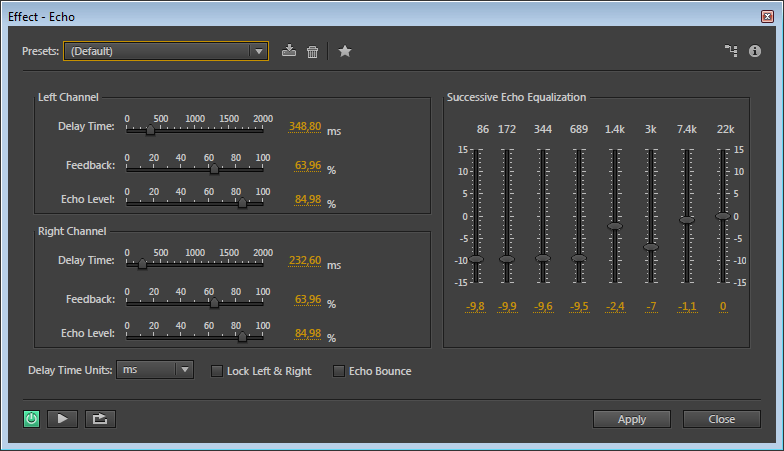
\includegraphics[width=0.75\textwidth]{pic-auecho-01}
  \caption{Окно Echo}
  \label{pic-auecho-01}
\end{figure}

Группа \emph{Successive Echo Equalization} представляет собой эквалайзер, с помощью которого можно изменять спектр задержанного сигнала.

\section{Реверберация}
\subsection{Распространение звука в замкнутом пространстве}
Распространение звуковых волн в замкнутом пространстве отличается от распространения звука в открытом пространстве. Попадая на поверхность, звуковая волна:
\begin{itemize}
  \item частично отражается от поверхности;
  \item частично поглощается материалом поверхности, переходя в тепловую энергию;
  \item незначительная ее доля проходит в соседнее помещение или пространство.
\end{itemize}

Какая именно часть энергии отражается обратно в помещение, определяет \textbf{коэффициент отражения} поверхности. Степень поглощения определяет \textbf{коэффициент поглощения}. Относительная мощность волны, прошедшей сквозь поверхность, задает \textbf{коэффициент звукопроводности}.

Рассмотрим пример: в комнате создается короткий акустический сигнал (рис. \ref{pic-acoustic-01}).
\begin{enumerate}
  \item Первым в точку приему \emph{Пр} придет прямой звук выстрела.
  \item Звуковые волны устремятся полу, потолку, стенам, предметам обстановки. Если отражающие поверхности находятся достаточно далеко от места выстрела и микрофона, то короткое время~--- единицы миллисекунд~--- микрофон ничего, кроме обычного шума помещения не уловит.
  \item К микрофону придут редкие и тихие единичные ранние отражения~--- по несколько штук от пола, потолка, стен. Ранние отражения распределятся по помещению равномерно.
  \item Возникнут взаимные переотражения, которые получили название поздних отражений. Они станут все чаще и сильнее, но не перестанут быть дискретными (раздельными). Средняя энергия звука (отзвука) в помещении продолжит увеличиваться и через 90..110 миллисекунд она достигнет максимума. По уровню этот максимум будет почти такой же, как и уровень прямого сигнала.
  \item После прохождения пика энергия начнет спадать, отражения будут становиться все более частыми, и через 150.. .300 миллисекунд они перестанут быть дискретными и станут диффузными, то есть взаимно переотраженными и перемешанными. При этом их уровень будет продолжать уменьшаться.
\end{enumerate}

\begin{figure}[h!]
  \centering
  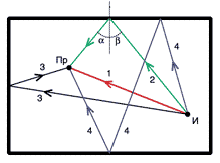
\includegraphics[width=0.75\textwidth]{pic-acoustic-01}
  \caption{Пример распространения звука в замкнутом пространстве}
  \label{pic-acoustic-01}
\end{figure}

На рис.  представлена \textbf{рефлектограмма} идеального помещения, на которой отображены:
\begin{itemize}
  \item кривая средней энергии сигнала;
  \item полоса, отображающая плотность отражений;
  \item варианты возможных отклонений параметров.
\end{itemize}
	
\begin{figure}[h!]
  \centering
  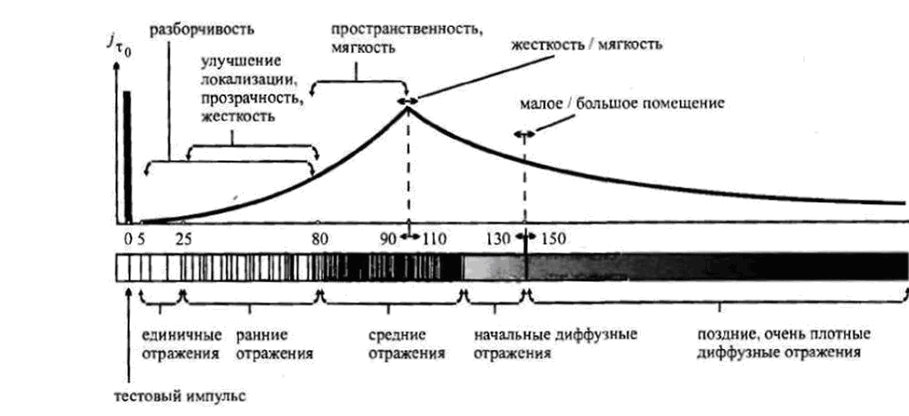
\includegraphics[width=0.95\textwidth]{pic-acoustic-02}
  \caption{Рефлектограмма идеального помещения}
  \label{pic-acoustic-02}
\end{figure}	

Свойства, которые наиболее сильно влияют на пространственные впечатления от реверберации:
\begin{itemize}
  \item процент прямого звука;
  \item процент ранних отражений, их пространственное распределение и время
  \item процент реверберационного хвоста, его пространственное распределение и время;
  \item длительность предварительной задержки (предзадержка);
\end{itemize}

Существуют помещения с мягким и жестким установлением звука. Если звук нарастает резко и через 90 миллисекунд достигает максимума акустика будет "<жесткой">. Если звук нарастает плавно и достигает максимума через 110 миллисекунд~---помещение будет "<мягким">.
\begin{itemize}
  \item Жесткое установление звука характеризуется большим уровнем прямого звука (как в передних рядах концертного зала) и сильными ранними отражениями. Такая акустика отличается высокой прозрачностью, четкостью, выразительностью, читаемостью отдельных нот и нюансов, но более заметны стилистические и интонационные погрешности исполнения.
  \item Мягкое установление характеризуется большей мощностью диффузного звука. При этом сглаживаются упомянутые шероховатости, увеличивается пространственное впечатление и ощущение параметров помещения.
\end{itemize}
	
Достаточно большое значение имеют координаты точки начала диффузных отражений: в малых помещениях они начинаются спустя 130 мс с момента тестового импульса, в больших~--- через 150 мс. Смещение этих значений в процессе создания модели искусственной реверберации может привести к появлению ощущения неестественности акустического отклика.

$RT_{60}$ (\emph{Reverb time})~--- \textbf{время реверберации},~--- время, необходимое для того, чтобы отражения звука уменьшились на 60 дБ ниже уровня прямого звука. Время реверберации зачастую устанавливают как одно значение, однако оно может быть измерено в разных частотных диапазонах сигнала (от 20 Гц до 20 кГц), или точнее в узких частотных полосах (одной октаве, $1/3$ октавы, $1/6$ октавы, и т.д.). Как правило, время реверберации измеряемое в узких частотных полосах будет отличаться в зависимости от частот содержащихся в полосе (высокие частоты затухают гораздо быстрее низких).

Оптимальное время реверберации зависит от типа музыки или звуков, которые должны звучать в пространстве. Помещения используемые для передачи речи, обычно требуют более короткого времени реверберации, для большей разборчивости слов. Если отраженный звук от одного слога слышен когда произносится следующий слог, то это может затруднить распознавание сказанного слова. Слова "<кот">, "<кол">, и "<ком"> могут быть очень похожи. С другой стороны, если время реверберации слишком коротко, то может пострадать тембровый баланс и громкость.

Основные факторы, влияющие на время реверберации, это размер и форма помещения, а также материалы, используемые при его строительстве. На время реверберации может повлиять любой объект помещённый в комнату, в том числе люди и их имущество.

Источник, издающий звук, отражается от различных поверхностей по-разному, в зависимости от их текстуры. Гладкие, жёсткие поверхности отражают звук подобно тому, как зеркало отражает свет (угол падения равен углу отражения). Тогда как отражение от грубых (неровных) материалов производится во многих направлениях, отражённый звук от таких поверхностей воспринимается более размытым. Характер отражений зависит от частоты звука и материала стен. Жёсткий материал поглощает звуковые волны меньше, тогда как мягкий больше.

Искажения позиционирования других точек, обозначенных на рефлектограмме (начало единичных отражений, появление ранних, средних и начальных диффузных отражений), не имеет решающего влияния на естественность акустической картины.

\subsection{Психоаккустические особенности восприятия пространства}
При определении направления и расстояния до источника звука используются следующие факторы:
\begin{itemize}
  \item амплитуда;
  \item время;
  \item тембр;
  \item отражения от ближайших поверхностей (реверберация).
\end{itemize}

\textbf{Амплитуда} является наиболее ясным и легче всего имитируемым параметром: чем громче звук, тем ближе его источник; чем громче звук в левом ухе, тем левее находится его источник. В современной звукозаписи эти факторы используются чаще всего~--- громкость звука увеличивается, чтобы вывести его на передний план (приблизить) и изменяется панорама (то есть увеличиваем громкость в одном канале стерео пары и уменьшаем в другом), чтобы переместить его влево или вправо.

Параметр \textbf{времени} также достаточно ясен~--- звук источника, расположенного слева, достигает левого уха на несколько микросекунд раньше, чем правого. Однако из-за очень малого времени задержки этот параметр практически невозможно имитировать на записи.

Изменение \textbf{тембра} в зависимости от расстояния происходит следующим образом~--- низкие частоты распространяются на более дальние расстояния, так что звуки, раздающиеся издалека, содержат меньше высоких частот. Воздействие тембра на направление сложнее~--- пока звук доходит от одного уха до другого, его тембр изменяется костями черепа и ушными раковинами. Попытка имитации этого эффекта называется \emph{head-related transfer function} (\emph{HRTF}). Она основана на субъективном восприятии многих людей, поскольку процесс этот еще недостаточно исследован и не может быть точно описан.

Если звук производится в помещении, то почти всегда кроме самого звука мы слышим и многочисленные его отражения (исключение составляют безэховые камеры).

Самыми важными при этом являются \textbf{ранние отражения}. В обычной прямоугольной комнате бывает от шести (пол, потолок и четыре стены) до десяти ранних отражений, прежде чем отражения начинают приходить столь часто, что сливаются в единую реверберацию.

\begin{figure}[h!]
  \centering
  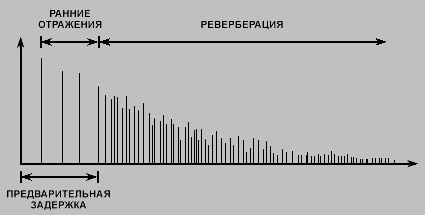
\includegraphics[width=0.75\textwidth]{pic-rever-01}
  \caption{Пример рефлектограммы помещения }
  \label{pic-rever-01}
\end{figure}	

Следует отметить, что ранние отражения воспринимаются нами не как повторения звука, а как информация об акустике помещения. Эта способность человеческого слуха называется "<\emph{эффект Хааса}"> по фамилии ученого, открывшего этот эффект в 1949 году. Ученый обнаружил, что если схожие звуки поступают с разных направлений с разницей по времени не более 50 миллисекунд, то мозг воспринимает только первый, более ранний звук, как отдельный, даже если последующие звуки громче первого на 10 дБ. Наш мозг автоматически объединяет прямой звук и его повторения, в результате мы слышим один звук, но обогащенный информацией об акустике помещения. Интересно, что совсем иначе воспринимаются звук и его повторения, если они поступают с одного направления.

Если просто объединить прямой звук и его задержанную копию, то произойдет изменение тембра звука, известное как результат действия "<гребенчатого фильтра">, то есть в определенном порядке одни частоты будут усилены, а другие ослаблены. Например, при объединении звука и его копии, задержанной на одну миллисекунду, будут усилены частоты 1 кГц, 2 кГц, 3 кГц и т. д., и ослаблены частоты 500 Гц, 1,5 кГц, 2,5 кГц и т. д. Однако в реальной жизни этого не происходит.

Наша система слуха устроена таким образом, что когда прямой звук и задержанный приходят с одного направления, то это воспринимается нами как информация о тембре, если же они приходят с разных направлений, то это воспринимается нами как информация о пространстве. Таким образом, если вы применяете небольшие по времени задержки (до 50 миллисекунд) для имитации акустики помещения, убедитесь, что прямой звук и задержанный разнесены по панораме. Кроме того, уровень ранних отражений обязательно должен быть как минимум на 6-10 дБ меньше прямого звука: во-первых, потому, что это соответствует реальным акустическим условиям, а, во-вторых, для снижения эффекта гребенчатого фильтра при монофоническом воспроизведении.

\begin{figure}[h!]
  \centering
  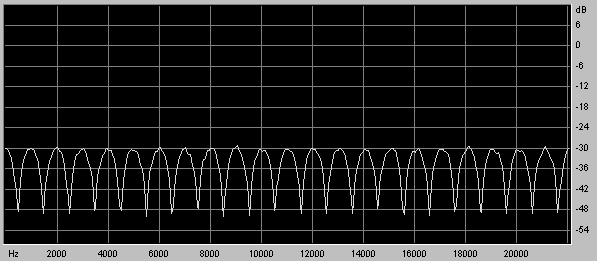
\includegraphics[width=0.95\textwidth]{pic-rever-02}
  \caption{Изменения тембра при наложении звука и его задержанной во времени копии}
  \label{pic-rever-02}
\end{figure}

Хотя большинство современных систем позиционирования звука в трехмерном пространстве используют изменения тембра, связанные с \emph{head-related transfer function}, эксперименты, проделанные специалистами по бинауральной записи показывают, что отражения (или реверберация) являются даже более важной составляющей процесса определения направления на источник звука, чем \emph{HRTF}.

В естественных условиях звук не всегда сопровождается реверберацией. Если мы находимся на открытом пространстве (по-английски это называется "<\emph{free field}">, что можно перевести как "<в чистом поле">), то звуку просто не от чего отражаться. Однако вся многовековая практика художественного исполнения, особенно музыкального, связана с помещениями, не просто обладающими реверберацией, но и использующими ее для усиления воздействия на слушателя.

\subsection{Применение реверберации}
С помощью реверберации можно создать эффект приближения и удаления источника звука. Для этого постепенно изменяют уровень реверберации, создавая иллюзию изменения звукового плана. При озвучивании фильмов или звуковом оформлении нередко возникает потребность подчеркнуть акустическую обстановку того или иного места действия. Для этого также используют эффект реверберации.

Эффект также очень часто используют для улучшения и подчеркивания художественной выразительности речи, вокала, звучания отдельных музыкальных инструментов. Реверберация может нести не только характер внешнего оформления, но и использоваться как средство усиления драматического действия. Например, шепот записанный с большим временем реверберации создаёт напряженный, пугающий эффект.

\textbf{Ревербератор} (англ. \emph{reverberator})~--- устройство или программа, имитирующая эффект реверберации. Реверберация, созданная с помощью таких устройств, называется искусственной, и может выполнять следующие задачи:
\begin{itemize}
  \item создание естественного пространственного эффекта;
  \item создание искусственных эффектов, которые не существуют в природе.
\end{itemize}

При создании эффекта сигнал изменяется так, что слушатель думает, что звук звучит в определенном пространстве (атмосфере), а не в "<сухой"> студии звукозаписи.

Первые эффекты реверберации создавались при помощи реального физического помещения, так называемых \textbf{эхо-камер} (рис. \ref{pic-echochamber-01}). В одном конце комнаты устанавливалась колонка, проигрывающая звук, а в другом микрофон, записывающий этот звук вместе с эффектом реверберации. Эта техника по прежнему используется, но она требует специальной звукоизоляции комнаты и создаёт одну из главных проблем~--- это трудность изменения времени реверберации.

\begin{figure}[h!]
  \centering
  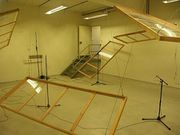
\includegraphics[width=0.6\textwidth]{pic-echochamber-01}
  \caption{Эхо-камера}
  \label{pic-echochamber-01}
\end{figure}

\textbf{Цифровые ревербераторы} для создания эффекта реверберации используют различные математические алгоритмы. Вследствие того, что реверберация вызвана очень большим количеством эхо, простые алгоритмы ревербераторов используют несколько схем задержек и обратной связи для создания больших, распадающихся серий эхо. Более продвинутые цифровые ревербераторы могут имитировать различные временные и частотные отклики реальных комнат.

С появлением цифровой обработки звука и других цифровых технологий стало возможным моделирование практически любой "<эхо-камеры">; по этой причине реверберационные комнаты перестали использоваться. Однако, естественно звучащие пространства, такие как церкви, продолжают использоваться в классической и других формах акустической музыки.

\textbf{Свёрточный (импульсный) ревербератор}~--- это цифровой процессор, моделирующий реверберацию физического или виртуального пространства на основе математической свёртки. В качестве свёртки используется предварительно записанный аудио сэмпл импульсного отклика моделируемого пространства. Процесс свёртки умножает каждый сэмпл звука для обработки (отражений) с сэмплами импульсного файла.

Основная цель импульсного ревербератора состоит в моделировании реального помещения, а именно~--- точное повторение реверберации определённой комнаты или устройства. При создании свёртки помещения в нём устанавливается микрофон или несколько микрофонов (для стерео эффекта), затем производится очень короткий импульс звука (часто электрической искры), микрофон улавливает все эти звуки, как оригинальный, так и отклик комнаты на этот звук (то есть реверберацию). Затем запись импульса очищается и загружается в процессор свертки (в импульсный ревербератор).

В сравнении с другими видами ревербераторов импульсный считается наиболее качественным. Потому как импульсы повторяют все особенности и нюансы помещений в которых они записывались. То есть если записать свёртку кафедрального собора, а потом этой свёрткой обработать звук, то его звучание будет помещено в этот собор, повторяя все его особенности. Более того, импульсы часто снимаются с дорогих аналоговых ревербераторов, такой импульс способен очень точно моделировать этот ревербератор без необходимости его покупки.

\begin{figure}[h!]
  \centering
  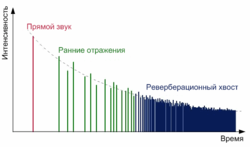
\includegraphics[width=0.75\textwidth]{pic-echochamber-02}
  \caption{Пример импульсной характеристика помещения}
  \label{pic-echochamber-02}
\end{figure}
	
Когда запись музыки в подавляющем большинстве случаев производилась в тех же помещениях, что и исполнение, и делалось это при помощи простых средств (например, двух микрофонов, установленных в зале), то есть запись была по сути документальной, то кроме звука инструментов и голосов записывались также и отражения. Результаты не были полностью идентичны реальному звучанию, поскольку микрофоны воспринимают звук не так, как человеческие уши, но все же некоторая доля естественной реверберации, а также информация о расположении источников звука на записи сохранялись.

Современная методика записи в большинстве случаев более искусственна (расположение микрофонов близко к инструментам, запись партий по отдельности, применение неакустических источников звука) и обычно никакой естественной реверберации на записи не содержится. Отсюда возникает потребность возместить потерю при помощи устройств искусственной реверберации.

Для того, чтобы применять ревербераторы, необходимо представить себе пространство, которое вы хотите имитировать, а также расположение в нем источника звука и слушателя.

\begin{itemize}
  \item
  Чем больше размеры помещения, тем больше время задержки ранних отражений и меньше их уровень.Чем больше размеры помещения, тем больше время предварительной задержки реверберации и меньше ее уровень.

  Время затухания реверберации не имеет прямой связи с размерами помещения (может быть короткая реверберация в большом, но хорошо заглушенном помещении, и наоборот), но, в большинстве случаев, чем больше помещение, тем дольше время реверберации. Последнее верно и для частотного состава реверберации: по идее, чем больше помещение, тем меньше уровень высоких частот, но этот параметр также связан с материалом поверхностей, а точнее их способностью поглощать разные частоты в разной степени.
  \item
  Чем больше расстояние от источника звука до слушателя, тем больше уровень ранних отражений и меньше время их задержки, а также тем больше уровень реверберации.

  При увеличении расстояния до источника звука прямой звук проходит больший путь и уровень его уменьшается. Отраженные звуки также проходят больший путь, однако это расстояние увеличивается меньше, чем расстояние для прямого звука, следовательно уровень отраженных сигналов уменьшается меньше, чем уровень прямого звука, и уровень отраженных сигналов по сравнению с уровнем прямого сигнала увеличивается.
\end{itemize}

Некоторые современные процессоры эффектов позволяют обойтись без напряжения пространственного воображения и предлагают формировать эффект, устанавливая размер помещения, расстояние до источника звука и выбирая материал стен, а все вопросы с ранними отражениями и реверберацией решаются этими процессорами самостоятельно.

\subsection{Эффекты реверберации в Adobe Audition}
В \emph{Adobe Audition} реализованы следующие эффекты реверберации:
\begin{itemize}
  \item \emph{Convolution Reverb}~--- позволяет создавать эффект реверберации на основе моделирования помещения с заданными характеристиками.
  \item \emph{Full Reverb}~--- эффект для моделирования реверберации с учетом размеров помещения, изменения спектра отраженно-го сигнала и т.д.
  \item \emph{Reverb}~--- позволяет моделировать реверберацию, но с меньшим количестом настроек, чем Full Reverb.
  \item \emph{Studio Reverb}~--- эффект для создания реверберации без моделирования помещения, за счет чего эффект получается менее требовательным к ресурсам процессора.
  \item \emph{Surround Reverb}~--- эффект для создания реверберации для звука в формате стерео 5.1.
\end{itemize}

Универсальная реверберация \emph{Full Reverb} используется в \emph{Adobe Audition} для того, чтобы в деталях моделировать акустическое пространство. Эффект обладает некоторыми уникальными возможностями:
\begin{itemize}
  \item реалистичное моделирование сигналов ранних отражений;
  \item изменение размеров и акустических свойств имитируемого помещения;
  \item моделирование любого материала отражающей поверхности;
  \item изменение поглощающих свойств пространства внутри помещения;
  \item коррекция частотного спектра сигнала реверберации с использованием трехполосного параметрического эквалайзера.
\end{itemize}

Эффект открывается командой \emph{Effects > Reverb > Full Reverb}, диалоговое окно содержит две вкладки: \emph{Reverb Settings} и \emph{Coloration}.

В группе \emph{Reverberation} имеются элементы регулировки общих параметров реверберации:
\begin{itemize}
  \item \emph{Decay Time}~--- общее время реверберации;
  \item \emph{Pre-Delay Time}~--- время достижения максимального уровня эффекта;
  \item \emph{Diffusion}~--- поглощающие свойства среды распространения звука;
  \item \emph{Perception}~--- характер восприятия реверберации: от размытого звука, характерного для его отражения от большого числа близко расположенных препятствий, до ясно различимого многократного эха;
\end{itemize}

\begin{figure}[h!]
  \centering
  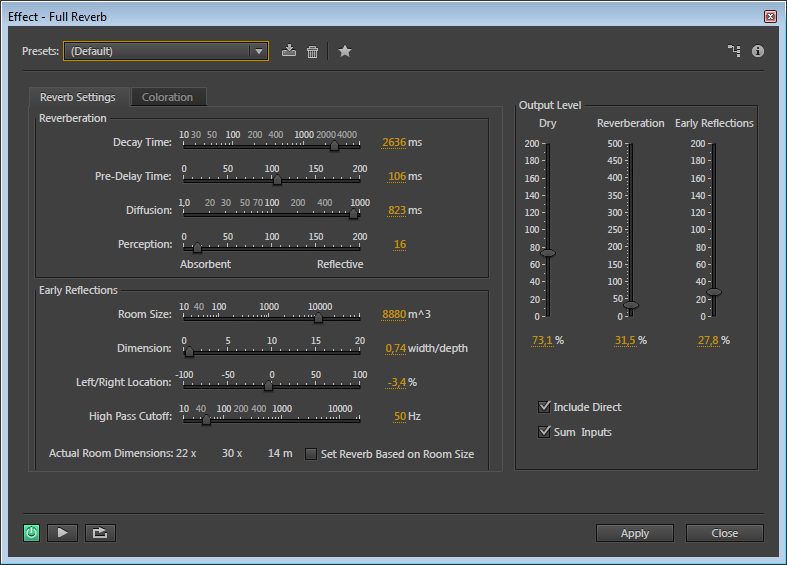
\includegraphics[width=0.75\textwidth]{pic-aureverb-01}
  \caption{Окно эффекта Full Reverb, закладка Reverb Settings}
  \label{pic-aureverb-01}
\end{figure}

\begin{figure}[h!]
  \centering
  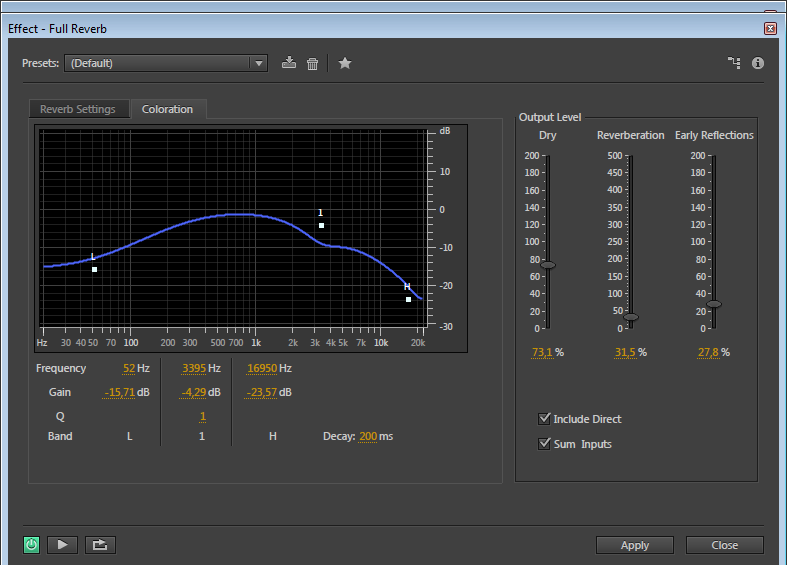
\includegraphics[width=0.75\textwidth]{pic-aureverb-02}
  \caption{Окно эффекта Full Reverb, закладка Coloration}
  \label{pic-aureverb-01}
\end{figure}

Параметры, устанавливаемые в группе \emph{Early Reflections}:
\begin{itemize}
  \item \emph{Room Size}~--- объем помещения в кубических метрах;
  \item \emph{Dimension}~--- отношение ширины помещения к длине;
  \item \emph{Left/Right Location}~--- точка локализации источника звука на стереопанораме;
  \item \emph{High Pass Cutoff}~--- частота среза фильтра высоких частот.
  \item \emph{Set Reverb based on Room Size}~--- автоматическое согласование общих параметров реверберации с параметрами ранних отражений, помещения и среды распространения.
\end{itemize}

В группе \emph{Output Level} имеются следующие элементы управления, которые регулируют:
\begin{itemize}
  \item \emph{Dry}~--- уровень необработанного сигнала;
  \item \emph{Wet (Reverb)}~--- уровень сигнала, обработанного эффектом.
  \item \emph{Wet (Early Reflections)}~--- уровень ранних отражений.
\end{itemize}

График на вкладке \emph{Coloration}~--- это амплитудно-частотная характеристика трехполосного параметрического эквалайзера, через который пропускается сигнал реверберации.

\subsection{Эффекты реверберации пакета Waves Platinum Native Bundle}
Эффект \emph{TrueVerb} создает реверберацию за счёт комбинации трёх компонентов звука: прямое звучание, ранние отражения и реверберация. Общий эффект процессора \emph{TrueVerb} зависит от баланса и характера этих трёх компонентов.

\begin{figure}[h!]
  \centering
  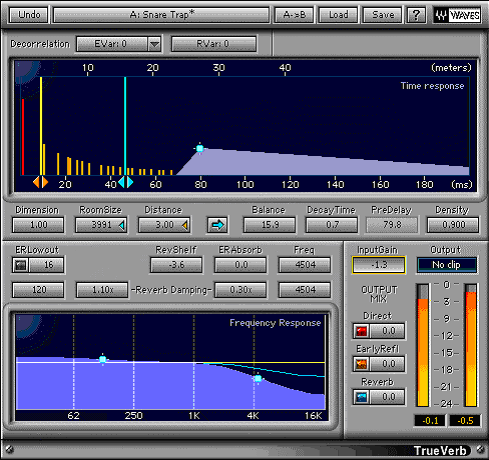
\includegraphics[width=0.75\textwidth]{pic-wavestrueverb-01}
  \caption{Окно эффекта True Verb}
  \label{pic-wavestrueverb-01}
\end{figure}

В верхней части окна (рис. \ref{pic-wavestrueverb-01}) на дисплее отображаются различные компоненты реверберирующего сигнала. Прямой сигнал отмечается красной вертикальной линией, расположенной в начале координат. Высота линии пропорциональна его уровню, зависящему от расстояния до источника звука. Оно в свою очередь отмечается на шкале вертикальной линией, цвет которой меняется от желтого (при небольших расстояниях до источника звука) до красного (когда расстояние близко к максимальному). Линию можно перемещать вправо или влево, ухватившись мышью за маркер, от которого она начинается, или, пользуясь кнопкой-слайдером \emph{Distance}. От этого параметра зависят также уровни ранних отражений (линии оранжевого цвета), и уровни реверберационного хвоста (закрашенная область светло-сиреневого цвета).

Еще одним параметром, влияющим на уровень прямого сигнала, является \emph{RoomSize} (размер помещения). От него зависит также плотность ранних отражений и уровень реверберации. На шкале графического дисплея RoomSize отмечается вертикальной линией голубого цвета.

Шкала над дисплеем отображает примерное расстояние (в метрах) до одной из отражающих поверхностей, то есть один из размеров помещения. Шкала под дисплеем позволяет оценить время ранних отражений в миллисекундах.

Кнопка-слайдер \emph{PreDelay} устанавливает задержку между прямым сигналом и началом реверберационного хвоста. На панели управления вы найдете кнопку в виде стрелки~---переключатель связанности параметров \emph{RoomSize} и \emph{PreDelay}. В связанном состоянии изменение одного параметра влечет за собой изменение другого в соответствии с акустическими свойствами помещения. При моделировании реальной акустики лучше установить связь параметров. В случае конструирования произвольного акустического пространства можно регулировать все по отдельности.
В левой нижней части окна расположен модуль эквалайзера. Его основным элементом является дисплей, на котором отображаются характеристики сразу двух фильтров: входного и выходного. При помощи входного фильтра можно осуществить предварительную коррекцию спектра входного сигнала. Выходной фильтр позволяет по отдельности регулировать скорость исчезновения низких и высоких частот из реверберирующего сигнала.

Плагин \emph{RVerb} (рис. \ref{pic-wavesrverb-01}) по своим возможностям подобен плагину \emph{TrueVerb}. Отличия заключаются в том, что характеристики входного и выходного фильтров ревербератора отображаются на различных дисплеях, кроме того, многие регуляторы выполнены в виде привычных и интуитивно понятных слайдеров.

\begin{figure}[h!]
  \centering
  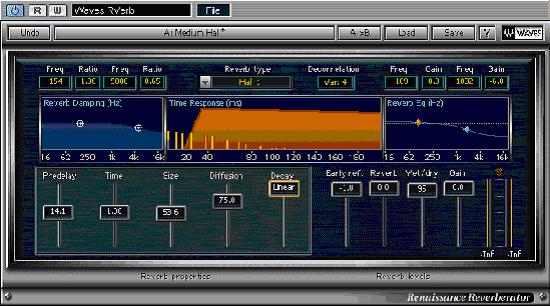
\includegraphics[width=0.75\textwidth]{pic-wavesrverb-01}
  \caption{Окно эффекта RVerb}
  \label{pic-wavesrverb-01}
\end{figure}

\section{Примеры использования эффектов дилей, эхо и реверберации}
Запись \emph{track01} содержит примеры применения эффекта \emph{Analog Delay} в режимах \emph{Tape}, \emph{Tube} и \emph{Analog}.

Запись \emph{track02} содержит примеры применения эффекта \emph{Echo}.

Запись \emph{track03} содержит примеры применения эффекта реверберации:
\begin{itemize}
  \item Часть 1 содержит два голоса, снятых на близкий микрофон в заглушённой студии.
  \item Часть 2 немного отличается: плотная реверберация имитирует большое, но поглощающее помещение, с близкими к камере голосами. Для большого и поглощающего помещения в части 2 ранние отражения начались в 40мсек и сгруппировались между 40 мсек и 100 мсек. Реверберационный хвост нарастает быстро, имеет широкую полосу и затухает через 0,3 секунды, микс был установлен на 40 процентов.
  \item Часть 3 соответствует меньшему помещению, но с более сильной реверберацией. Ранние отражения находятся между 16 мсек и 40 мсек. Реверберационный хвост также нарастает быстро и имеет около 0,7 секунды затухания, хотя высокие частоты затухают немного быстрее. Так как эта реверберация длиннее, то микс отчасти меньше: с использованием тех же настроек, что и в части 2, он был равен 25 процентам.
  \item Реверберационный хвост средней длины может помочь монтажным участкам музыки, позволяя инструментам затухать естественным образом через монтажный стык. Такая реверберация представлена в части 4. Вы, возможно, даже не заметите ее, когда играет музыка, но можете услышать ее в двух местах, когда музыка внезапно останавливается. Ранние отражения находятся в первых 50 мсек, затем реверберационный хвост очень быстро нарастает и имеет 3,3 секунды затухания. Микс равен 35 процентам.
  \item В части 5 находятся голоса, звучащие внутри большого стального бака. Здесь нет ранних отражений, а реверберационный хвост начинается со средней скоростью атаки через несколько миллисекунд после прямого звука. Но хотя высокие частоты затухают примерно через две секунды, низким частотам для этого необходимо около 10 секунд.
  \item Вы можете добавить предварительную задержку для имитации огромного пространства. В результате получилась довольно хорошая железнодорожная система громкого оповещения, приведенная в части 6.
  \item Добавьте ФВЧ примерно на 500 Гц, чтобы имитировать потери в сети передачи сообщений, и она будет близкой к совершенству (часть 7). 
\end{itemize}

\end{document}

